\chapter{Training Procedure and Mechanisms}
\label{chap:training-system}

\definecolor{tsEnc}{HTML}{2E6DB4}
\definecolor{tsDec}{HTML}{E08A2E}
\definecolor{tsNew}{HTML}{2E9E5B}
\definecolor{tsAcc}{HTML}{7B4FB0}
\definecolor{tsGray}{HTML}{8A8A8A}

Chapter~\ref{chap:architectures} fixed the network architecture and, with it, the capacity and inductive biases available to the agent. Architecture alone does not determine behavior: the training procedure decides which of those biases are used and how. Two agents sharing the same \code{UECD} backbone can learn very different policies depending on the reward components they receive, the opponents they train against, and the schedule controlling the exploration-exploitation trade-off.

This chapter specifies the training procedure built on top of \code{UECD}. The mechanisms are presented in conceptual order, from those closest to per-step action sampling to those targeting global generalization. Figure~\ref{fig:training-pipeline} offers a complementary view along a different axis: it places each group on the PPO data-flow loop, with each tag pointing to the stage it modifies. Section~\ref{sec:training-algo} defines the PPO baseline used by every experiment. Section~\ref{sec:action-sampling} refines how the factored action is sampled and credited. Section~\ref{sec:reward-signal} groups the eight mechanisms acting on the reward and value signals that feed the PPO update. Section~\ref{sec:opponent-curriculum} handles non-stationarity from multiple opponents. Section~\ref{sec:representation} adds auxiliary supervision to the shared encoder. Section~\ref{sec:generalization} covers symmetry and multi-map training. Section~\ref{sec:arch-enhancements} closes with two architectural refinements evaluated alongside the training features rather than the architectures of Chapter~\ref{chap:architectures}. Every mechanism is gated by CLI flag and disabled by default (Table~\ref{tab:training-catalog}), supporting the controlled feature ablation reported in Chapter~\ref{chap:results}.
         
\vspace{-0.3em}

\section{PPO Baseline Configuration}
\label{sec:training-algo}

All agents train with the PPO~\cite{schulmanProximalPolicyOptimization2017}  loop of Section~\ref{sec:ppo-overview}. The baseline uses PPO-Clip (Equation~\ref{eq:ppo-loss}) with GAE~\cite{schulmanHighDimensionalContinuousControl2015} (Equation~\ref{eq:gae}); Table~\ref{tab:baseline-config} lists the full configuration.

\vspace{-0.7em}

\begin{table}[H]
\centering
\caption[Baseline PPO hyperparameters]{Baseline PPO hyperparameters used by every experiment of Chapter~\ref{chap:results} when no flag-gated mechanism is active. Experiment-specific settings (map, opponents, hardware) appear there.}
\label{tab:baseline-config}
\small
\begin{tabularx}{\textwidth}{@{}l l X@{}}
\toprule
\textbf{Hyperparameter} & \textbf{Value} & \\
\midrule
\multicolumn{3}{@{}l}{\textbf{\emph{PPO objective}}}\\
Discount $\gamma$ / GAE $\lambda$  & $0.99\,/\,0.95$ & \\
Clip range $\epsilon$              & $0.1$ & \\
Value loss coefficient $c_v$       & $0.5$ & \\
Entropy coefficient $\beta$        & $0.01 \to 0.001$ & \textit{linearly annealed (Section~\ref{sec:reward-signal})} \\
\midrule
\multicolumn{3}{@{}l}{\textbf{\emph{Stabilization}}}\\
Learning rate                      & $2.5 \times 10^{-4} \to 0$      & \textit{linearly annealed to prevent late-training oscillations} \\
Max gradient norm                  & $0.5$                                          & \textit{prevents destabilizing updates} \\
Advantage normalization & per-minibatch & \textit{prevents single-episode gradient domination} \\
\midrule
\multicolumn{3}{@{}l}{\textbf{\emph{Rollout and batch}}}\\
Rollout length $T$                 & $512$ & \\
Update epochs / minibatches        & $2\,/\,3$ & \\
Parallel environments              & $24$ & \\
Batch size                         & $12\,288$ & \\
\bottomrule
\end{tabularx}
\end{table}

\begin{figure}[!htb]
\centering
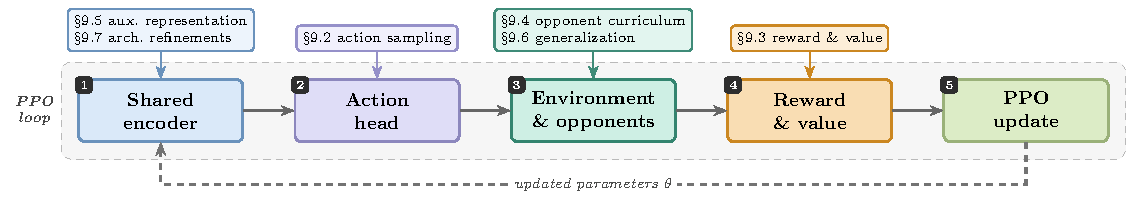
\includegraphics[width=\linewidth]{chapters/09_training_system/figures/training_pipeline.pdf}
\caption[Training mechanisms on the PPO loop]{Each training mechanism acts on one stage of the PPO loop. The boxes form the core loop of Figure~\ref{fig:microrts-ppo-loop} in data-flow order; the tags above each box name the sections modifying it.}
\label{fig:training-pipeline}

\vspace{2em}

\captionof{table}[Catalog of flag-gated training mechanisms]{Training mechanisms introduced in this chapter, each gated by a CLI flag and disabled by default. Only the principal flag per mechanism is listed; secondary flags tuning internal hyperparameters keep their defaults. The final group lists observation and environment features from Chapter~\ref{chap:python_bridge}, included here for the feature ablation in Chapter~\ref{chap:results}.}
\label{tab:training-catalog}
\footnotesize
\begin{tabularx}{\textwidth}{@{}l l c X@{}}
\toprule
\textbf{Mechanism} & \textbf{CLI flag} & \textbf{Section} & \textbf{Acts on} \\
\midrule
\multicolumn{4}{@{}l}{\textbf{\emph{Action sampling}}}\\
Autoregressive head      & \texttt{--autoregressive}        & \ref{sec:action-sampling}  & sub-action logits \\
Hierarchical masking     & \texttt{--hierarchical-mask}     & \ref{sec:action-sampling}  & log-prob \& entropy terms \\
\midrule
\multicolumn{4}{@{}l}{\textbf{\emph{Reward and value signal}}}\\
Entropy scheduling       & \texttt{--ent-coef-end}          & \ref{sec:reward-signal}    & entropy bonus \\
Reward scheduling        & \texttt{--reward-schedule}       & \ref{sec:reward-signal}    & reward weight vector \\
Multi-phase schedule     & \texttt{--phase-steps}           & \ref{sec:reward-signal}    & LR / entropy / blend / vf coef per phase \\
Build-time rewards       & \texttt{--reward-unit-build-time}& \ref{sec:reward-signal}    & production reward \\
Decomposed value heads   & \texttt{--triple-value-heads}, \texttt{--advantage-weights} & \ref{sec:value-heads} & critic / advantage blend \\
PopArt normalization     & \texttt{--popart}                & \ref{sec:reward-signal}    & value targets \\
HL-Gauss value           & \texttt{--hl-gauss}              & \ref{sec:reward-signal}    & value loss \\
PAE   & \texttt{--pae-keep}              & \ref{sec:reward-signal}    & advantage estimate \\
\midrule
\multicolumn{4}{@{}l}{\textbf{\emph{Opponent curriculum and self-play}}}\\
Adaptive opponents       & \texttt{--adaptive-opponents}    & \ref{sec:opponent-curriculum} & env opponent mix \\
Historical self-play     & \texttt{--num-selfplay-envs}, \texttt{--pfsp} & \ref{sec:opponent-curriculum} & env opponents \\
MCW        & \texttt{--prioritized-sampling}  & \ref{sec:opponent-curriculum} & policy-gradient weights \\
\midrule
\multicolumn{4}{@{}l}{\textbf{\emph{Auxiliary representation}}}\\
Spatial ownership        & \texttt{--aux-spatial}           & \ref{sec:representation}   & shared encoder \\
Unit count               & \texttt{--aux-unit-count}        & \ref{sec:representation}   & shared encoder \\
Temporal contrastive     & \texttt{--aux-contrastive}       & \ref{sec:representation}   & shared encoder \\
Opponent action modeling & \texttt{--aux-opponent-modeling} & \ref{sec:representation}   & shared encoder \\
\midrule
\multicolumn{4}{@{}l}{\textbf{\emph{Generalization and architecture}}}\\
Symmetry augmentation    & \texttt{--augment-symmetry}      & \ref{sec:generalization}   & observations / masks \\
Multi-map + PLR          & \texttt{--multi-map}, \texttt{--plr} & \ref{sec:generalization} & map sampling \\
GELU activation          & \texttt{--gelu}                  & \ref{sec:arch-enhancements}& encoder / decoder \\
SPP critic               & \texttt{--spp-critic}            & \ref{sec:arch-enhancements}& critic pooling \\
\midrule
\multicolumn{4}{@{}l}{\textbf{\emph{Observation and environment (introduced in Chapter~\ref{chap:python_bridge})}}}\\
Extended observations (73ch)  & \texttt{--extended-obs}          & \ref{sec:obs-encoding}  & observation encoding \\
Filtered masks + reserved obs & \texttt{--filtered-masks}, \texttt{--reserved-obs} & \ref{sec:action-space} & action mask / observation \\
Frame stacking                & \texttt{--frame-stack}           & \ref{sec:wrappers}      & observation history \\
\bottomrule
\end{tabularx}
\end{figure}


\section{Action Sampling Refinements}
\label{sec:training-enhancements}
\label{sec:action-sampling}

The factored action head of Section~\ref{sec:action-space} produces $\lvert \mathtt{nvec} \rvert = 7$ sub-action logits per cell, sampled independently and summed uniformly in the PPO loss. Two refinements modify this default. \emph{Autoregressive sampling} introduces dependencies between sub-actions; \emph{hierarchical masking} removes the credit signal of semantically inactive sub-actions. Both alter the policy objective without changing the rollout: the same actions are sampled and dispatched to the engine, only the way logits are produced and credited changes.

\paragraph{Autoregressive sub-action sampling.}

Sub-actions are not independent: when a unit chooses \emph{produce}, the production direction and unit type should be jointly coherent. Following the autoregressive action decomposition of AlphaStar~\cite{vinyalsGrandmasterLevelStarCraft2019}, an autoregressive head conditions each sub-action on the previously sampled ones via learned embeddings. The standard per-component logit $\ell_k = W_k \cdot \mathbf{f} + b_k$ becomes
\begin{align}
\ell_k = W_k \cdot [\,\mathbf{f},\; e_1(a_1),\; \ldots,\; e_{k-1}(a_{k-1})\,] + b_k,
\end{align}
where $\mathbf{f}$ is the per-cell spatial feature vector from the actor's pre-projection layer and $e_j(\cdot)$ is a learned embedding of dimension $d_e = 8$ for sub-action $j$. The first sub-action (\code{action\_type}) is conditioned only on $\mathbf{f}$. The factorization is intra-unit: inter-unit dependencies still flow indirectly through the shared spatial and entity representations of Chapter~\ref{chap:architectures}.

\paragraph{Hierarchical sub-action masking.}

For any given \code{action\_type}, only a subset of the seven sub-actions is semantically active (Figure~\ref{fig:hier-mask}). When an agent selects \emph{attack}, the sub-actions for \emph{move direction}, \emph{harvest direction}, \emph{return direction}, \emph{produce direction}, and \emph{produce unit type} have no effect on the environment. The standard implementation~\cite{huangGym$m$RTSAffordableFull2021} nevertheless aggregates all seven log-probabilities and entropies into the PPO objective, diluting credit assignment across non-informative sub-actions. Following RAISocketAI~\cite{goodfriendCompetitionWinningDeep2024}, a hierarchical sub-action mask zeroes out the log-probability of each conditional sub-action when its parent \code{action\_type} is inactive. Unlike the invalid-action mask of Section~\ref{sec:action-space}, which prevents illegal actions at the environment level, this mask operates purely on the PPO objective: the contributions of semantically inactive sub-actions are zeroed in the loss. Let $a_0 \in \{0,1,2,3,4,5\}$ denote the chosen \code{action\_type} and let $\textsc{parent}(k)$ map sub-action $k$ to its activating type:
\[
\textsc{parent}(k) =
\begin{cases}
\texttt{MOVE}    & k=1 \\
\texttt{HARVEST} & k=2 \\
\texttt{RETURN}  & k=3 \\
\texttt{PRODUCE} & k=4 \\
\texttt{PRODUCE} & k=5 \\
\texttt{ATTACK}  & k=6
\end{cases}
\]
Sub-action $k{=}0$ (the \code{action\_type} itself) is always active. The masked log-probability becomes
\begin{align}
\log \pi(\mathbf{a} \mid s)
  = \log \pi_0(a_0 \mid s)
    + \sum_{k=1}^{6} m_k \, \log \pi_k(a_k \mid s, a_{<k}),
\end{align}
where $m_k = \mathbbm{1}\!\left[\,a_0 = \textsc{parent}(k)\,\right] \in \{0,1\}$ gates sub-action $k$ on its parent. The same gating applies to the per-sub-action entropy terms. The credit signal becomes cleaner: the distribution over \emph{move direction} updates only when the unit actually moves, rather than receiving phantom gradients during attack, harvest, or production steps.

\begin{figure}[H]
    \centering
    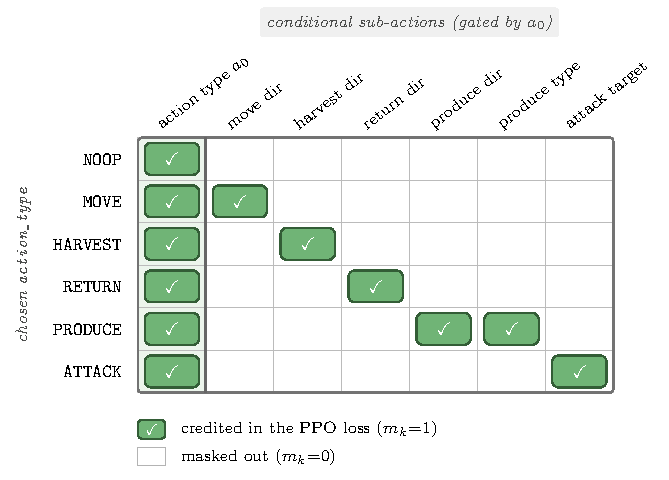
\includegraphics[width=0.75\linewidth]{chapters/09_training_system/figures/hier_mask.pdf}
    \caption[Hierarchical sub-action masking]{Hierarchical sub-action masking. Rows are the chosen \code{action\_type} $a_0$; columns are the seven sub-actions. A filled cell marks a sub-action credited in the PPO objective; an empty cell is masked out ($m_k = 0$). Only \code{action\_type} is always credited; each conditional sub-action contributes under its single parent, so each row credits at most three of the seven sub-actions.}
    \label{fig:hier-mask}
\end{figure}

\vspace*{-0.6cm}

\section{Reward and Value Signal}
\label{sec:reward-signal}
The PPO objective depends on two scalar signals per transition: the reward $r_{t+1}$ feeding the policy gradient through the GAE advantage, and the bootstrapped value $V(s_t)$ that grounds the critic's update. Eight mechanisms refine how these scalars are constructed, scaled, or weighted. The first four reshape the policy update signal: entropy regularization, dense-to-sparse annealing, multi-phase scheduling, and build-time weighting; the next two restructure the value function (decomposed heads, PopArt); the last two are experimental alternatives: HL-Gauss for the value loss and the PAE for the GAE advantage.

\vspace{-0.2cm}

\subsection*{Reshaping the Reward}

\paragraph{Entropy scheduling.}

The entropy bonus $H[\pi_\theta]$ in the PPO objective (Equation~\ref{eq:ppo-loss}) is controlled by a coefficient $\beta$, linearly annealed to a configurable end value via the scheduler below. This encourages exploration early, then shifts toward exploitation as the policy matures.

\paragraph{Reward scheduling and multi-phase training.}

Dense reward signals accelerate early learning but risk producing policies that over-optimize intermediate proxies at the expense of the true objective, a phenomenon formally established by~\cite{ngPolicyInvarianceReward1999}. RAISocketAI~\cite{goodfriendCompetitionWinningDeep2024} addresses this in MicroRTS with a shaped-to-sparse transition~\cite{huangActionGuidanceGetting2020}. A piecewise-linear scheduler (Figure~\ref{fig:schedule-engine}) generalizes this transition: given $N$ phases with plateau values $[v_1, v_2, \ldots, v_N]$ and boundary steps $[s_1, e_1, s_2, e_2, \ldots]$, each hyperparameter holds $v_i$ until step $s_i$, interpolates linearly to $v_{i+1}$ by step $e_i$, then holds $v_{i+1}$ until the next transition. The dense-to-sparse transition uses this scheduler to interpolate the reward weights from the dense configuration of Table~\ref{tab:reward-functions} to the sparse win/loss configuration $[10, 0, \ldots, 0]$ over $[t_{\text{start}}, t_{\text{end}}]$ (by default, $30$\% to $70$\% of training), shifting from ``play economically well'' toward ``win the game''. The same scheduler drives the learning rate, entropy coefficient, advantage blend weights, and value loss coefficients, enabling multi-stage curricula within a single run.

\vspace{-0.3cm}

\begin{figure}[!htb]
    \centering
    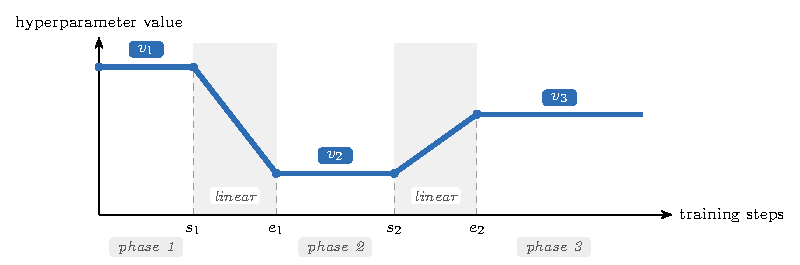
\includegraphics[width=\linewidth]{chapters/09_training_system/figures/schedule_engine.pdf}
    \caption[Piecewise-linear multi-phase scheduler]{Piecewise-linear multi-phase scheduler. Each hyperparameter holds plateau value $v_i$ until step $s_i$, interpolates linearly to $v_{i+1}$ by step $e_i$, then holds again. The same scheduler drives the reward weights (dense-to-sparse), learning rate, entropy coefficient, and value-head weights.}
    \label{fig:schedule-engine}
\end{figure}

\vspace{-0.3cm}

\paragraph{Build-time-scaled unit production rewards.}

The default reward function assigns the same weight ($4.0$) to producing any military unit. These units have very different production costs in game ticks: Light (80), Ranged (100), Heavy (120). Uniform weighting biases the policy toward cheap units regardless of tactical fit. Following RAISocketAI~\cite{goodfriendCompetitionWinningDeep2024}, this mechanism scales each production reward by build time, using $(4.0, 5.25, 6.0)$ for (Light, Ranged, Heavy). The Light and Heavy weights are strictly proportional to build time; Ranged receives an extra $0.25$ for its long-range advantage.

\subsection*{Restructuring the Value Function}

\paragraph{Decomposed value heads.}
\label{sec:value-heads}

A single value function struggles to track the shifting reward signal: the critic must estimate returns from dense shaping rewards and sparse win/loss signals at different discount horizons. Up to three independent critic heads decouple this target~\cite{vanseijenHybridRewardArchitecture2017}, following RAISocketAI~\cite{goodfriendCompetitionWinningDeep2024} (Table~\ref{tab:value-heads}). Each head receives its own per-step reward: \emph{shaped} sums the $9$ components of Section~\ref{sec:reward-functions}; \emph{sparse} uses only Win/Draw/Loss; \emph{cost} uses the temporal difference of the normalized Military score. Each head computes advantages via a separate GAE pass (Equation~\ref{eq:gae}) and is trained with its own value loss.

The per-head advantages live in the natural scale of their reward signals, which differ substantially. To make contributions comparable, each advantage is z-scored per minibatch (zero mean, unit variance) before being combined into a single advantage driving the policy gradient:
\begin{align}
\hat{A} = w_{\text{sh}} \cdot \hat{A}_{\text{shaped}}
        + w_{\text{sp}} \cdot \hat{A}_{\text{sparse}}
        + w_{\text{co}} \cdot \hat{A}_{\text{cost}},
\qquad w_{\text{sh}} + w_{\text{sp}} + w_{\text{co}} = 1.
\end{align}

\begin{table}[!htb]
\centering
\caption[Value head configuration]{Value head configuration. Higher $\gamma$ and $\lambda$ capture longer-horizon dependencies. Blend weights $w$ sum to $1$; value-loss coefficients $c_v$ scale each head's contribution to the total loss.}
\label{tab:value-heads}
\small
\begin{tabularx}{\textwidth}{@{}l X c c c l@{}}
\toprule
\textbf{Head} & \textbf{Reward signal} & $\boldsymbol{\gamma}\,/\,\boldsymbol{\lambda}$ & $\boldsymbol{w}$ & $\boldsymbol{c_v}$ & \textbf{Role} \\
\midrule
Shaped  & Weighted sum of all $9$ components (Table~\ref{tab:reward-functions}) & 0.99\,/\,0.95  & 0.5 & 0.5 & Dense feedback \\
Sparse  & Win\,/\,Draw\,/\,Loss only                              & 0.999\,/\,0.99 & 0.3 & 0.1 & Terminal outcome \\
Cost    & Temporal $\Delta$ of Military score$^{\dagger}$ & 0.999\,/\,0.99 & 0.2 & 0.2 & Army strength proxy \\
\bottomrule
\multicolumn{6}{p{\textwidth}}{\footnotesize $^{\dagger}$\,Cost-head reward $r^{\text{co}}_t = s_t - s_{t-1}$, the temporal difference of the normalized Military score $s_t = \frac{S_{\text{own}} - S_{\text{opp}}}{S_{\text{own}} + S_{\text{opp}} + 1} \in (-1, +1)$, where $S = \sum_{\text{units}} \text{cost} \times (1 + \text{HP}/\text{HP}_{\max})$ is the player's total army value (cost-weighted, HP-adjusted). $s_{t-1} = 0$ at the start of each episode.} \\
\end{tabularx}
\end{table}

\paragraph{PopArt value normalization.}

When the reward signal varies across orders of magnitude, as in reward scheduling with a shifting target distribution, standard Mean Squared Error (MSE) value loss can produce destabilizing gradient spikes. Preserving Outputs Precisely, while Adaptively Rescaling Targets (PopArt)~\cite{vanhasseltLearningValuesMany2016} keeps a running mean $\mu$ and standard deviation $\sigma$ of value targets via EMA:
\begin{align}
\mu_{\text{new}} = (1 - \alpha) \cdot \mu_{\text{old}} + \alpha \cdot \bar{G}_{\text{batch}}, \qquad \sigma^2_{\text{new}}=(1-\alpha)\sigma^2_{\text{old}}+\alpha \cdot \overline{(G-\bar G_{\text{batch}})^2},
\end{align}
with smoothing factor $\alpha = 3 \times 10^{-4}$. The critic learns to predict in a normalized space $\hat{V}_{\text{norm}} \approx \mathcal{N}(0,1)$, and predictions are denormalized for GAE computation:
\begin{align}
\hat{V}(s) = \sigma \cdot \hat{V}_{\text{norm}}(s) + \mu.
\end{align}
On each update of $\mu$ and $\sigma$, the last linear layer's weights and bias are simultaneously rescaled so the denormalized output $\hat{V}(s)$ remains identical for every $s$. The network's predictions thus stay continuous when the normalization statistics change, preserving training stability. When multiple value heads are active, PopArt is applied independently to each.

\subsection*{Experimental Alternatives}

\paragraph{Value estimation via classification (HL-Gauss).}

Histogram Loss with Gaussian Targets (HL-Gauss)~\cite{imaniImprovingRegressionDistributional2018}, recently applied to DRL value estimation by~\cite{farebrother2024StopRegressing}, is included as an experimental alternative to scalar value regression. It discretizes the value range into $255$ uniformly spaced bins and predicts a categorical distribution over them. Returns are first compressed via the symmetric logarithm $\text{symlog}(x) = \text{sign}(x) \cdot \ln(|x|+1)$ from DreamerV3~\cite{hafnerMasteringDiverseDomains2023}, mapping large values into $[-10, 10]$. Target labels are Gaussian distributions centered on the compressed return with width $\sigma_{\text{HL}} = 0.75$:
\begin{align}
p_i^{\text{target}} \propto \exp\!\left(-\frac{(c_i - \text{symlog}(G_t))^2}{2\sigma_{\text{HL}}^2}\right),
\end{align}
where $c_i$ is the $i$-th bin center. The loss is the cross-entropy between predicted logits and these soft targets. At inference, the scalar value is recovered as
\begin{align}
\hat{V}(s) = \text{symexp}\!\left(\sum_i p_i \cdot c_i\right).
\end{align}
This formulation bounds gradient magnitudes (cross-entropy is bounded, unlike MSE), naturally handles multimodal return distributions, and is more robust to non-stationary targets. The bin count and symlog range are kept at their published defaults rather than tuned to the MicroRTS return scale, a choice revisited when the ablation evaluates this feature in Chapter~\ref{chap:results}.

\paragraph{Partial Advantage Estimator.}

When PPO collects fixed-length trajectory segments of $T$ steps that do not reach a terminal state, GAE estimates near the segment's end suffer from high bias: fewer future TD residuals and an inaccurate bootstrap value $V(s_T)$. The Partial Advantage Estimator (PAE)~\cite{jinPartialAdvantageEstimator2025} addresses this by zeroing advantages for the last $(1{-}\kappa) \cdot T$ steps of incomplete segments, so only the first $\lfloor \kappa \cdot T \rfloor$ steps contribute to the policy gradient (Figure~\ref{fig:pae}). Segments containing a terminal state are used in full, since the terminal reward eliminates bootstrap bias. The value function is still trained on all steps, since even slightly biased return targets remain informative for regression. This matters in MicroRTS, where episodes last $3\,000$ to $8\,000$ steps but rollouts collect only $T = 512$, so most segments are incomplete. Despite using fewer transitions per update, PAE is reported to improve win rates in MicroRTS in its originating work~\cite{jinPartialAdvantageEstimator2025}; the ablation of Section~\ref{sec:feat-ablation} re-examines this on the present setup ($\kappa = 0.95$).

\begin{figure}[!htb]
    \centering
    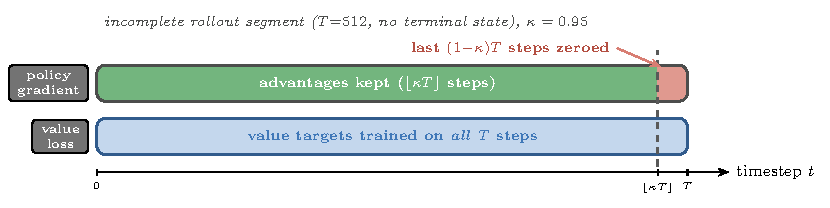
\includegraphics[width=\linewidth]{chapters/09_training_system/figures/pae.pdf}
    \caption[PAE on an incomplete rollout segment]{PAE on an incomplete rollout segment ($T = 512$, $\kappa = 0.95$). Advantages are zeroed for the last $(1-\kappa)T$ steps where the inaccurate bootstrap $V(s_T)$ would propagate bias through GAE; only the first $\lfloor \kappa T \rfloor$ steps drive the policy gradient (green). The value loss uses all $T$ steps (blue), since even biased return targets remain informative for regression.}
    \label{fig:pae}
\end{figure}

\section{Opponent Curriculum and Self-Play}
\label{sec:opponent-curriculum}

Training against a fixed scripted opponent leads to overfitting to a single strategy. By default, bot environments are distributed across a fixed diverse pool, emphasizing two strong opponents (CoacAI and Mayari) while retaining exposure to simpler strategies (RandomBiasedAI, WorkerRush, LightRush). This fixed mix is the baseline of Chapter~\ref{chap:results}. Three mechanisms layer on top of it. \emph{Adaptive scheduling} replaces the fixed mix with a difficulty-progression curriculum; \emph{historical self-play with PFSP} adds past agent versions as opponents; \emph{Matchup Competitiveness Weighting} reweights transitions according to opponent difficulty within the PPO update itself. The last two are orthogonal to the bot pool and combine with either the fixed mix or the adaptive curriculum.

\paragraph{Adaptive opponent scheduling.}

When adaptive scheduling is enabled, all bot environments start against RandomBiasedAI. An \code{AdaptiveOpponentScheduler} tracks per-opponent win rates over a sliding window (default: $50$ games) and escalates the difficulty (Figure~\ref{fig:opponent-curriculum}). When the agent surpasses a threshold win rate (default: 70\%) against the currently trained bot, the matching environments are promoted to the next tier. A minimum of two environments per tier is kept to prevent forgetting earlier strategies. The interaction with self-play is gated. While the terminal tier is not yet mastered, the self-play environments remain dormant: their transitions are filtered from the PPO update and their results ignored by every scheduler. When all terminal-tier opponents reach a configurable mastery threshold (default: 90\%), the dormant environments switch to PFSP-hard sampling against historical checkpoints while the adaptive bot curriculum continues in parallel. The result is a fully automated curriculum, from a single easy bot through scripted-bot mastery to self-play, without manual intervention. When enabled, this adaptive curriculum replaces the fixed baseline mix entirely; the two are mutually exclusive.

\begin{figure}[!htb]
    \centering
    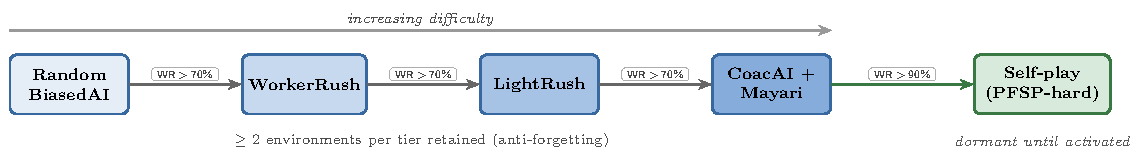
\includegraphics[width=\linewidth]{chapters/09_training_system/figures/opponent_curriculum.pdf}
    \caption[Automated opponent curriculum]{Automated opponent curriculum. Each bot environment is promoted to the next tier once its sliding-window win rate exceeds 70\%, with at least two environments per tier kept to prevent forgetting. Self-play stays dormant until every terminal-tier opponent is mastered, then switches to PFSP-hard sampling against historical checkpoints.}
    \label{fig:opponent-curriculum}
\end{figure}

\paragraph{Historical self-play and PFSP.}

Once scripted opponents are mastered, training against them yields diminishing returns. Self-play~\cite{zhangSurveySelfplayMethods2025} exposes the agent to an opponent that adapts alongside it. A \code{CheckpointPool} stores every saved checkpoint and, at each refresh, builds a candidate set from all \emph{recent} checkpoints (a First-In First-Out (FIFO) buffer of the last $k$) plus a uniform subsample of \emph{historical} ones, balancing recency with diversity. A subset of environments plays against a checkpoint sampled from this set, refreshed every $M$ updates. Pool sampling follows three modes inspired by PFSP~\cite{vinyalsGrandmasterLevelStarCraft2019}: \code{uniform} (random selection), \code{hard} ($P \propto (1-\mathrm{WR})^p$, prioritizing opponents the agent loses to), and \code{var} ($P \propto \mathrm{WR} \cdot (1-\mathrm{WR})$, prioritizing uncertain 50/50 matchups). In the feature ablation of Section~\ref{sec:feat-ablation}, self-play uses \code{hard} mode with the default exponent $p = 1.0$ (reducing to $P \propto 1 - \mathrm{WR}$); the sampled opponent is refreshed every $M = 50$ updates (${\approx}600$\,\text{k} environment steps), drawn from a pool split evenly between the recent and historical buffers.

\paragraph{Matchup Competitiveness Weighting.}

Matchup Competitiveness Weighting (MCW) is a novel transition-level reweighting scheme operating within the PPO minibatch update. PFSP samples opponents by win-rate proximity~\cite{vinyalsGrandmasterLevelStarCraft2019}, and Prioritized Experience Replay (PER) weights transitions off-policy by TD-error~\cite{schaulPrioritizedExperienceReplay2015}. MCW combines both ideas but operates on-policy and at transition level, preserving the rollout distribution. The distinction from PFSP variants is deliberate: a competitiveness-weighted PFSP scheme ($P \propto \mathrm{WR}(1-\mathrm{WR})$) reweights the probability of sampling an opponent and thereby changes which data is collected, whereas MCW leaves the rollout distribution untouched and reweights only each transition's gradient contribution inside the update. The two act on orthogonal axes, data collection vs gradient weighting, and could in principle be combined. An \code{OpponentTracker} maintains per-opponent win rates over a sliding window (default: $100$ games), and each transition receives weight
\begin{equation}
w_k = 1 - |\mathrm{WR}_k - 0.5|,
\label{eq:mcw}
\end{equation}
where $\mathrm{WR}_k \in [0,1]$ is the sliding-window win rate against opponent $k$. The weight peaks at $\mathrm{WR}_k = 0.5$ (value $1.0$) and decays linearly to $0.5$ at $\mathrm{WR}_k \in \{0, 1\}$, a $2{:}1$ ratio between fully competitive and fully decided matchups (Figure~\ref{fig:mcw-weight}). Weights are then renormalized so that $\bar{w}=1$ across the rollout, preserving the gradient's overall magnitude.

\begin{figure}[!htb]
    \centering
    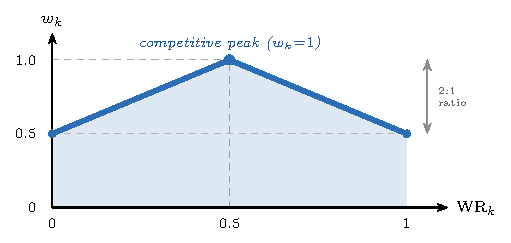
\includegraphics[width=0.75\linewidth]{chapters/09_training_system/figures/mcw_weight.pdf}
    \caption[MCW transition weight vs win rate]{MCW transition weight $w_k = 1 - |\mathrm{WR}_k - 0.5|$ as a function of the sliding-window win rate against opponent $k$. The weight peaks at $1.0$ for even matchups and decays to $0.5$ for fully decided ones (a $2{:}1$ ratio), then is renormalized to mean $1$ over the rollout.}
    \label{fig:mcw-weight}
\end{figure}

MCW reweights \emph{only the policy-gradient term} of the PPO objective; the entropy bonus and the value losses of all critic heads (shaped, sparse, cost) remain uniform across transitions:
\begin{equation}
\mathcal{L} = \mathbb{E}_t\bigl[\,w_t\,\mathcal{L}^{\text{CLIP}}(t)\,\bigr]
- \beta \,\mathbb{E}_t[\mathcal{H}(\pi_t)]
+ \sum_{h \in \{\text{sh},\text{sp},\text{co}\}} c_{\text{v},h}\,\mathbb{E}_t[\mathcal{L}^{\text{VF},h}(t)],
\label{eq:ppo-with-mcw}
\end{equation}
where $w_t$ is the MCW weight assigned to transition $t$, $\mathcal{L}^{\text{CLIP}}$ the standard PPO clipped surrogate (Equation~\ref{eq:ppo-clip}), $\mathcal{H}(\pi_t)$ the policy entropy with coefficient $\beta$  (Equation~\ref{eq:entropy-bonus}), and $\mathcal{L}^{\text{VF},h}$ the value loss of critic head $h \in \{\text{shaped}, \text{sparse}, \text{cost}\}$ weighted by $c_{\text{v},h}$  (Equation~\ref{eq:value-loss}). Only the surrogate term carries the per-transition weight $w_t$; all other terms aggregate uniformly over the batch. This decoupling is intentional: the value heads must produce unbiased estimates across the full opponent distribution for the GAE advantages to remain well calibrated, while the policy update concentrates its capacity on the most informative signal (near-$50$\% matchups). The triangular weight itself is a design choice rather than a derived optimum: any profile that peaks at even matchups and decays toward decided ones would serve the same role, and tuning its exact shape is left to future work.

\section{Auxiliary Representation Learning}
\label{sec:representation}

The PPO reward signal alone may not push the encoder to capture all strategically relevant features. Four auxiliary heads share the encoder with the actor and critic, training jointly with the PPO objective to add gradient signal that shapes internal representations. Table~\ref{tab:aux-tasks} summarizes the four heads; architectural details and strategic rationale follow.

\begin{table}[!htb]
\centering
\caption[Auxiliary prediction heads]{Auxiliary prediction heads sharing the \code{UECD} encoder.}
\label{tab:aux-tasks}
\footnotesize
\begin{tabularx}{\textwidth}{@{}l X X X@{}}
\toprule
\textbf{Head} & \textbf{Architecture} & \textbf{Target} & \textbf{Loss} \\
\midrule
Spatial ownership        & $1{\times}1$ conv                                & Per-cell P0 / P1 ownership map           & Binary cross-entropy (per cell) \\
Unit count               & AdaptiveAvgPool $\to$ MLP                         & 12-d vector (6 types $\times$ 2 players) & MSE \\
Temporal contrastive     & Pool $\to$ MLP $\to$ 128-d $\ell_2$ embedding     & Same vs other timesteps in batch         & InfoNCE (Information Noise-Contrastive Estimation)~\cite{oordRepresentationLearningContrastive2018} \\
Opponent action modeling & Conv head, per enemy cell                         & Enemy action type (6 classes)            & Focal cross-entropy ($\gamma_f=2$)~\cite{linFocalLossDense2017} \\
\bottomrule
\end{tabularx}
\end{table}

\emph{\textbf{(i)} Spatial ownership} forces the encoder to explicitly represent territorial control, a key strategic concept in RTS games. Targets are downsampled when the encoder resolution differs from the observation resolution. \emph{\textbf{(ii)} Unit count} maintains a global summary of army composition, information otherwise distributed across spatial positions and essential for production and engagement decisions. \emph{\textbf{(iii)} Temporal contrastive learning} pulls embeddings of consecutive timesteps $t$ and $t{+}1$ together (positive pair) while pushing them away from other environments in the batch (negatives). In MicroRTS, consecutive states are highly correlated (units move one cell per action), so capturing this continuity helps the encoder distinguish meaningful state changes from noise. \emph{\textbf{(iv)} Opponent action modeling} predicts each enemy unit's next action type (None, Move, Harvest, Return, Produce, Attack); the focal loss downweights easy predictions (e.g., idle units) and focuses on informative ones (e.g., attacking or producing units), encouraging the encoder to reason about opponent intentions.

\medskip

The four heads differ in convergence behavior. Spatial ownership and unit count can in principle reach zero loss, since the agent observes the full game state and the targets are deterministic functions of the observation. Opponent action modeling and temporal contrastive learning are inherently noisy: the opponent's actions depend on its internal policy (unobservable), and consecutive states may differ unpredictably. For the latter two, the goal is not zero loss but a useful gradient signal that shapes the encoder representations throughout training.

The total loss combines the PPO objective with the per-task auxiliary losses:
\begin{align}
\mathcal{L}_{\text{total}} = \mathcal{L}_{\text{PPO}} + \sum_i c_i \cdot \mathcal{L}_{\text{aux},i},
\end{align}
with per-task coefficients $c_i$ (defaults: $0.1$ for spatial ownership and unit count, $0.05$ for temporal contrastive and opponent action modeling).

\section{Generalization}
\label{sec:generalization}

Two mechanisms target generalization at different levels: \emph{symmetry augmentation} exploits within-map invariances, while \emph{multi-map training} exposes the policy to different maps in one run.

\paragraph{Symmetry augmentation.}

Most MicroRTS maps are spatially symmetric, yet a CNN trained on a fixed orientation may learn position-dependent biases (e.g., always expanding leftward). The \code{SymmetryAugmentation} wrapper (Section~\ref{sec:wrappers}) assigns each environment one of four flip modes at episode start (identity, horizontal flip, vertical flip, or $180^\circ$ rotation), consistently transforming observations, action masks, and the $7{\times}7$ attack target grid. Applied only during training, the augmentation quadruples positional diversity without extra rollouts. It is most natural on symmetric maps, where each flipped observation corresponds to an equivalent game state; on asymmetric maps (e.g., \emph{BWDistantResources32x32}, \emph{BloodBath.scmB}), it changes the orientation distribution and should be interpreted as data augmentation rather than an exact game symmetry.

\paragraph{Multi-map training and Prioritized Level Replay.}

The padded environment of Section~\ref{subsec:padding} enables training across maps from $8{\times}8$ to $64{\times}64$ within a single run. Two scheduling strategies are available. \emph{Cyclic rotation} rotates maps every $M$ updates (default: $50$) in round-robin order. \emph{Prioritized Level Replay} (PLR)~\cite{jiangPrioritizedLevelReplay2021} samples the next map proportionally to learning difficulty, $P(\text{map}_i) \propto (1 - \mathrm{WR}_i) + \epsilon$ (with $\epsilon = 0.1$), allocating more training time to maps where the agent currently struggles.

\section{Architectural Refinements}
\label{sec:arch-enhancements}

The two final modifications operate on the activation function and the critic's pooling layer respectively. They affect the optimization landscape and value estimation rather than the network's representational capacity, so they are evaluated alongside the training features in Chapter~\ref{chap:results} rather than the architecture ablation.

\paragraph{GELU activation.}

All ReLU activations in the encoder and decoder can be replaced with GELU (Gaussian Error Linear Unit)~\cite{hendrycksGaussianErrorLinear2016}:
\begin{align}
\text{GELU}(x) = x \cdot \Phi(x),
\end{align}
where $\Phi$ is the standard Gaussian cumulative distribution function. Unlike ReLU, GELU provides a smooth, non-zero gradient for negative inputs. In the \code{UECD} architecture, which stacks $14$ CBAM-ResBlocks, smooth gradients can reduce dead neurons and improve convergence.

\paragraph{SPP critic.}

The default critic uses adaptive average pooling to reduce the encoder output to a fixed-size vector. The Spatial Pyramid Pooling (SPP)~\cite{heSpatialPyramidPooling2015} variant replaces this with multi-scale pooling: the feature map is pooled at three resolutions ($1{\times}1$, $2{\times}2$, $4{\times}4$) and the results concatenated, providing global and local spatial information regardless of map size. This matters for multi-map training (Section~\ref{sec:generalization}), where a single critic must evaluate positions on maps from $8{\times}8$ to $64{\times}64$~\cite{lemosEnhancingDeepReinforcement2025}.